\begin{figure}[ht!]
	\begin{minipage}{0.48\linewidth}
		\centering
		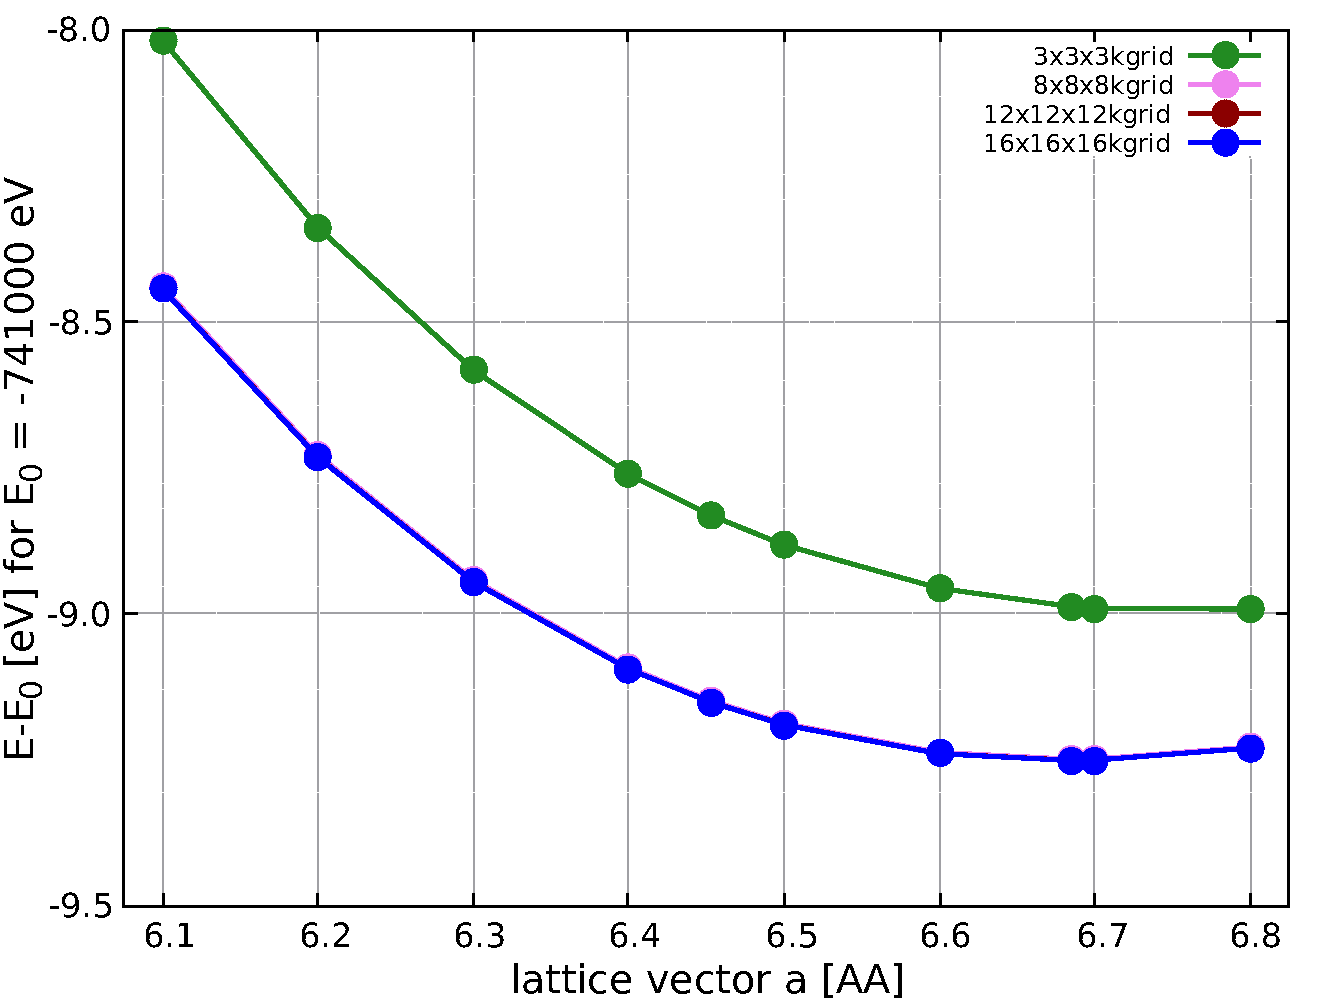
\includegraphics[width=\linewidth]{andere_bilder/plot_energies_hgte_bulk_all_kgrid_in_one.pdf}
		\caption{Lattice constant $a$ with respect to the total energy, calculated with four different k-grids. Lines for k-grids 8x8x8, 12x12x12 and 16x16x16 are overlaid.}\label{kgrid_lattice_constant}
	\end{minipage}
	\hfill
	\begin{minipage}{0.48\linewidth}
		\centering
		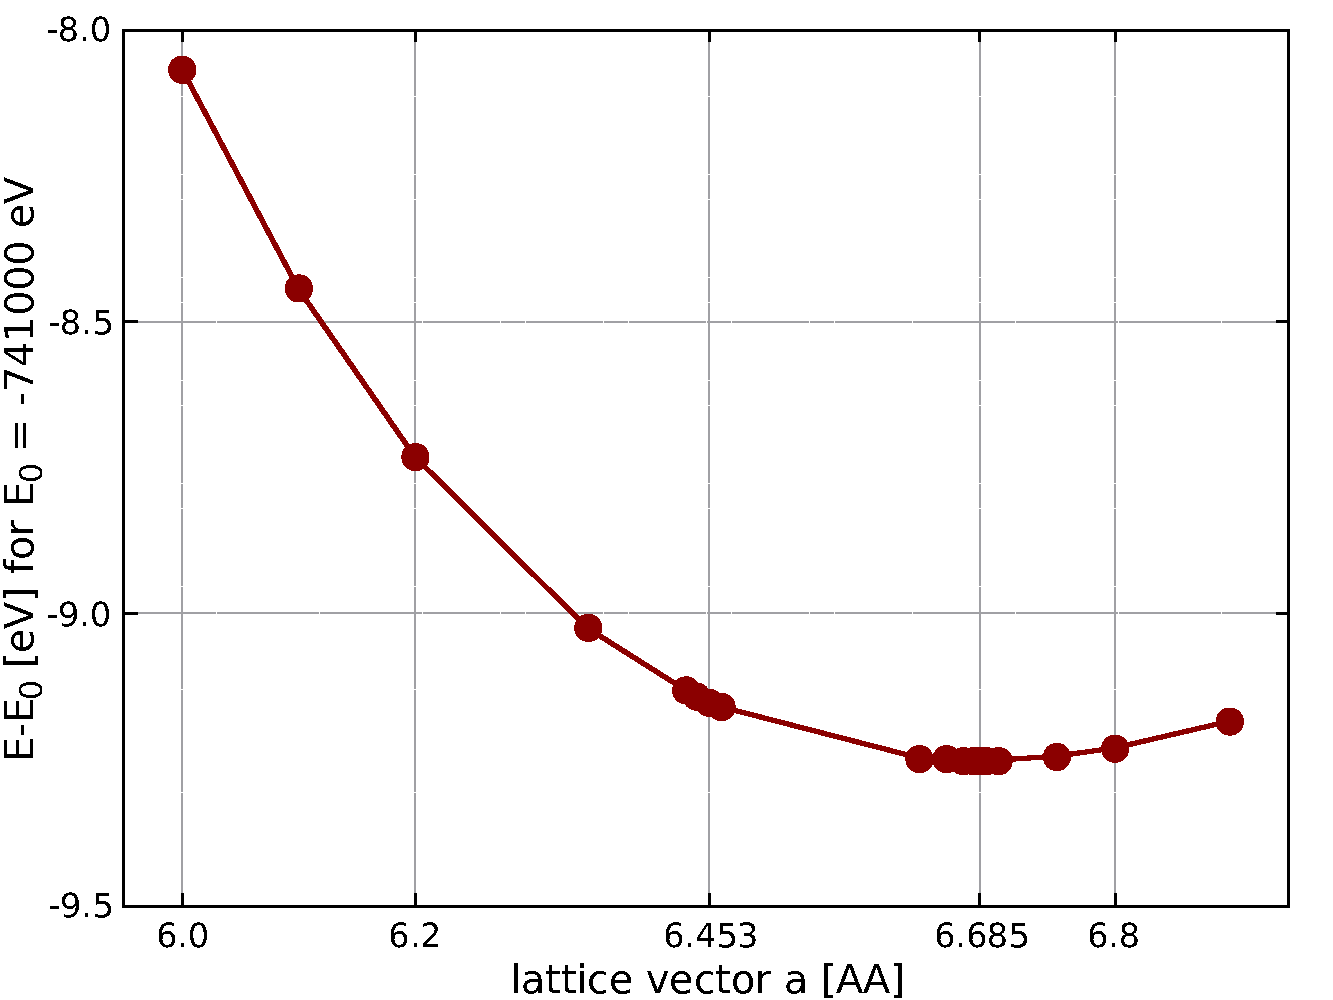
\includegraphics[width=\linewidth]{andere_bilder/lattice_constant_study_spin_none_no_soc.pdf}
		\caption{Lattice constant $a$ with respect to the total energy. The lowest energy was found for 6.685 Angström.}\label{lattice_constant}  \vspace{12.5pt}
	\end{minipage}
\end{figure}

	First of all the lattice constant $a$ with the lowest total energy in the HgTe bulk must be determined, since the energetically most stable constitution of a crystal structure is given by the smallest total system energy respective to the lattice constant.  
%because this one will be the most stable lattice constant.
	Both the bulk and the slab calculations must have the right values for the the k-grid density in order to make calcutions faster and less computanionally expensive. 		
%At the same time, the bulk calculations, and also the ones for the surface, are in need of the right choice of the k-grid parameters. 

	In figure \ref{kgrid_lattice_constant} one can see the result for lattice vector $a$ in Angström with respect to the total energy of the bulk, with different k-grids. It is clear, that 3x3x3 gives no representative results. 
%Here the lattice constant also doesn't have a minimum. 

	After carefully looking at the results of the energy convergence tests, the lattice constant was determined by using a higher k-grid than 8x8x8 to be sure about the convergence of the calculations. The result of the final step to determine the best theoretical value of the lattice constant for our crystal structure can be seen in figure \ref{lattice_constant}.
%	and the one with the lowest energy was 6.685 Angström. 
	As one can see, the best results were obtained for a lattice constant of 6.685 Angstrom.

%	Then the k-grid study was done again just for this lattice constant. In figure \ref{k_grid_study} there is the outcome of the bulk k-grid and additionally the ones for 4 layers, 8 layers and 16 layers. And now it makes sense that in figure \ref{kgrid_lattice_constant} that above 8 the graphs are identical. The energy doesn't change for higher k-grids. 
	It is this lattice constant, that was used for executing a detailed k-grid study. The results of this study is shown in figure \ref{k_grid_study} where additionally the results for the slabs with 4, 8 and 16 layers are illustrated.  
	It is not surprising that the most economic values of the k-grids for the slabs are virtually the same as for the bulk namely around 12x12x12. But since for higher k-grids the band structure curve becomes smoother, we used 24x24x24 in order to get smooth results. 
	Note that although the CPU time therefore increases, this is not significant for the calculations of the systems regarded in this thesis. 
%	For the slabs the graphs look a bit different. The convergence is not as smooth as for the bulk and the k-grid must be higher for a physical output. 
%	Theoretically, the higher the k-grid, the smoother the band structure or dos output. But the CPU time is also increasing. This means, one has to choose a k-grid some where in the middle. I used 24 points per direction for all following calculations. 
\begin{figure}[b!]
	\begin{subfigure}[c]{.5\linewidth}
		\centering
		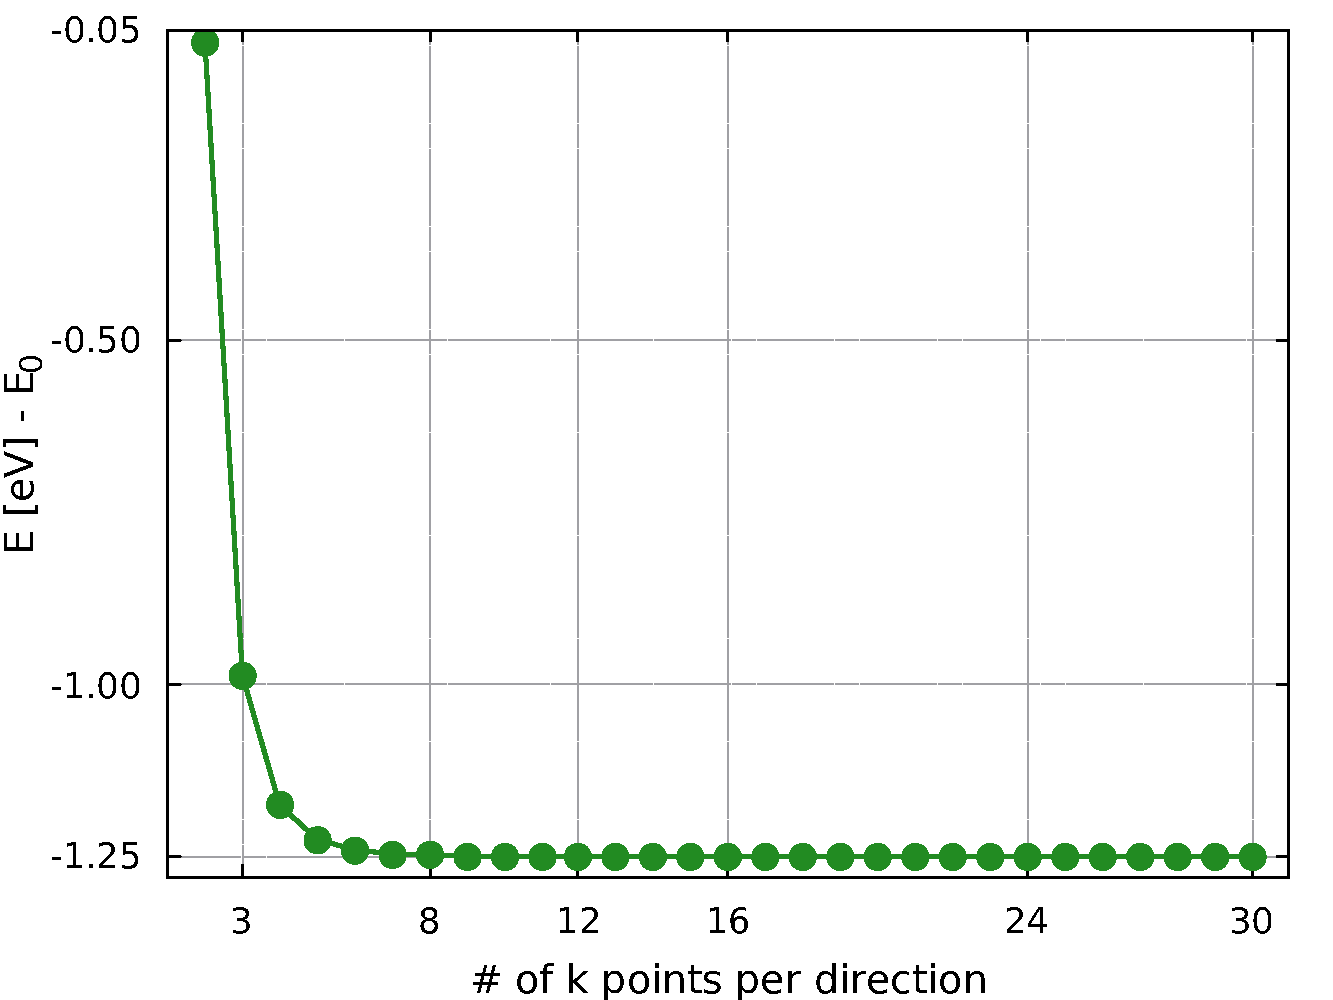
\includegraphics[width=\linewidth]{andere_bilder/kgrid_bulk.pdf}
		\caption{Bulk with $E_0= -741008 \,\unit{eV}$} \label{k_grid_1}
		\vspace{5pt}
	\end{subfigure}
	\hfill
	\begin{subfigure}[c]{.5\linewidth}
		\centering
		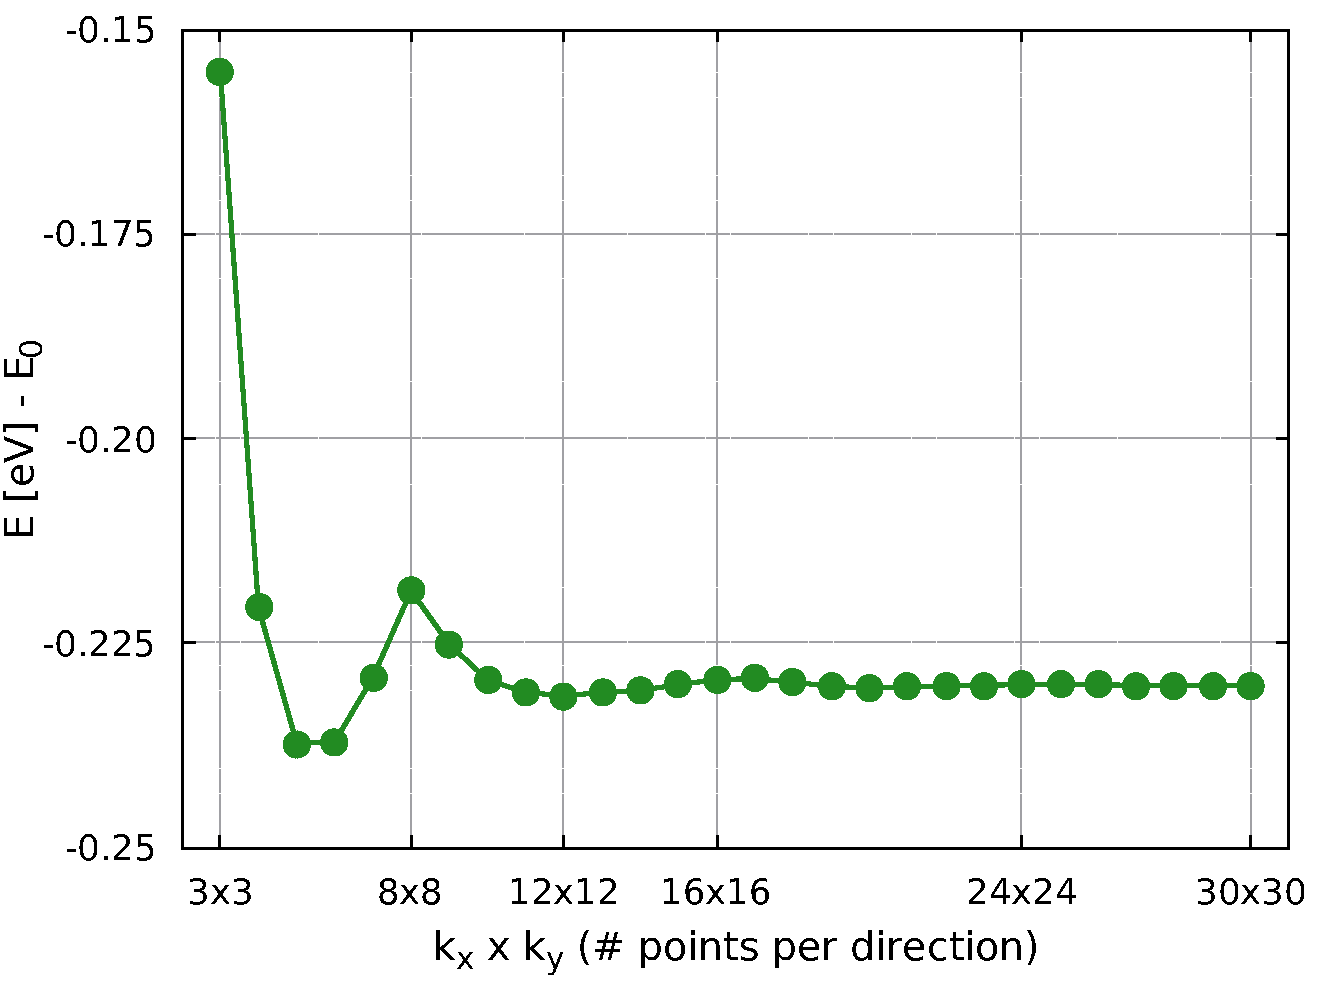
\includegraphics[width=\linewidth]{andere_bilder/kgrid_1x1x4_layers.pdf}
		\caption{Slab with 4 layers with $E_0= -1482047 \,\unit{eV}$} \label{k_grid_2}
		\vspace{5pt}
	\end{subfigure}
	\begin{subfigure}[c]{.5\linewidth}
		\centering
		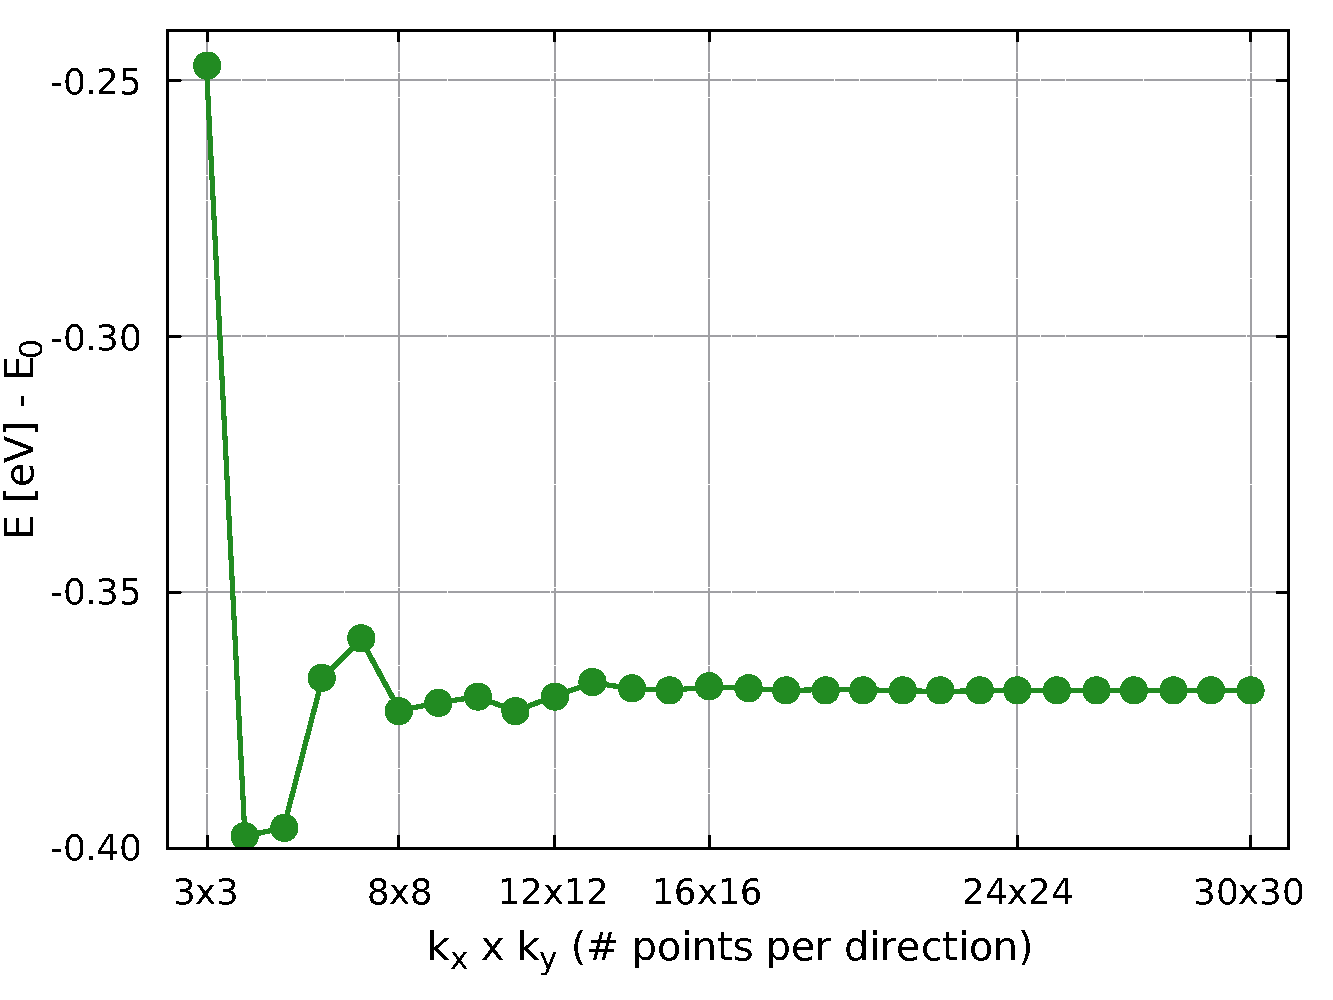
\includegraphics[width=\linewidth]{andere_bilder/kgrid_1x1x8_layers.pdf}
		\caption{Slab with 8 layers with $E_0= -2964065 \,\unit{eV}$} \label{k_grid_3}
	\end{subfigure}
	\hfill
	\begin{subfigure}[c]{.5\linewidth}
		\centering
		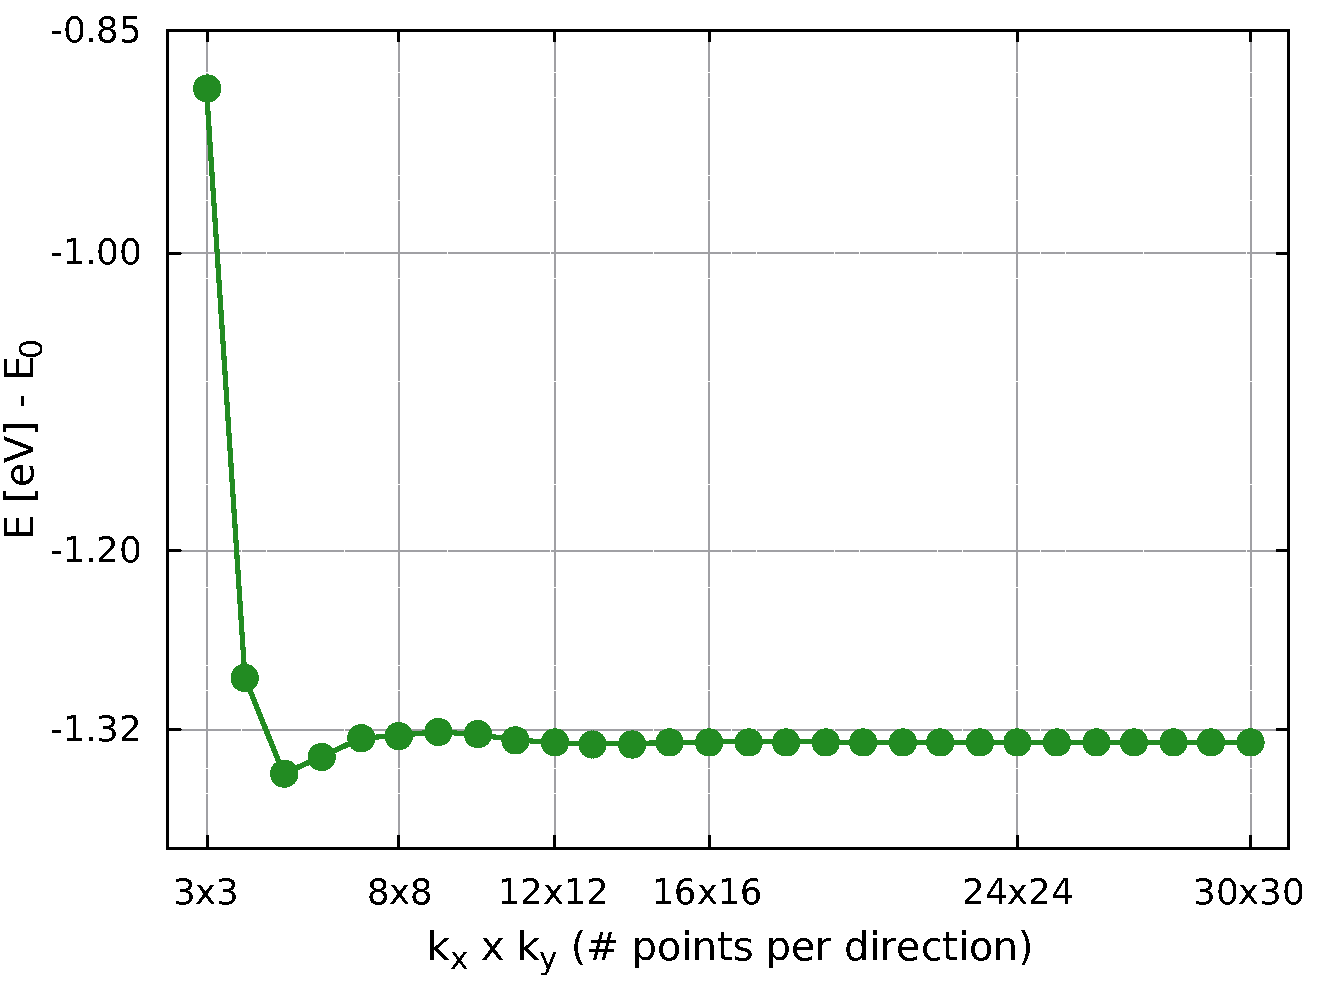
\includegraphics[width=\linewidth]{andere_bilder/kgrid_1x1x16_layers.pdf}
		\caption{Slab with 16 layers with $E_0= -5928101 \,\unit{eV}$} \label{k_grid_4}
	\end{subfigure}
	\caption{Total energy $E [\unit{eV}] - E_0$ (with $E_0$ the energy offset) as a function of k-grid spacing.} \label{k_grid_study}
\end{figure}

\FloatBarrier	
	%%% Local Variables:
	%%% mode: latex
	%%% TeX-master: "main_BA2.0"
	%%% End: